\documentclass[../report.tex]{subfiles}

\begin{document}
\section{Factory Patterns}
Redegøre for opbygningen af GoF Fatory og Abstract Factory Pattern.
\\

De to patterns hører til Creational Patterns kategorien, hvor deres generelle ide er faktorisering ved at sepererer oprettelse af objektet fra dens anvendelse. De bruges til at kontrollerer klasse initialisering.

\subsection*{Factory Pattern}
Dette pattern definerer et interface for oprettelse af objektet, man lader klassen der implementerer interfacet bestemmet, hvilket objekt der skal oprettes. Dvs. at den i princippet er en udskifter for en klasse constructor.

\begin{figure}[H]
    \centering
    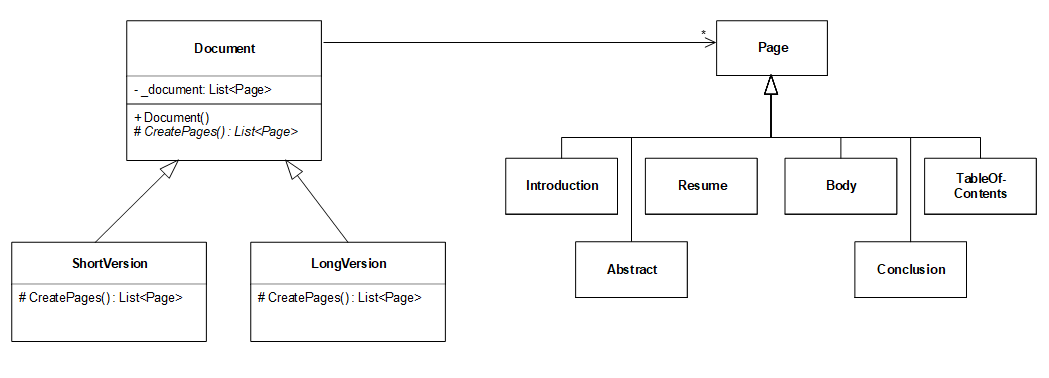
\includegraphics[width = \textwidth]{pics/factory_pattern.PNG}
    \caption{Factory Pattern}
    \label{fig:factory_pattern}
\end{figure}

Definerer et interface ud fra \textbf{CreatePage()}, men lader klasserne der implementerer interfacet bestemme hvilket objekt der skal oprettes. Den abstrakte klasse vil blive anvendt således, at andre funktioner kan modtages ved arv af subklasserne.

\subsection*{Abstract Factory Pattern}
Det abstrakte factory pattern giver mulighed for, at oprette grupper af relaterede objekter, uden krav om at angive de nøjagtive konkrete klasser, der vil blive anvendt.
\\

Abstract Factory er godt hvis man gerne vil generaliserer et system. Et eksempel kunne være et vægtsystem. Har man f.eks. et vægtsystem, der kun virker for Føtex, og der senere skal kunne inarbejdes et ny system ved siden af, skal der ændres i mange ting. Dvs. godt til store og komplekse systemer.


\begin{figure}[H]
    \centering
    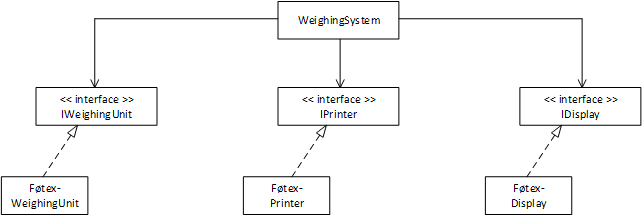
\includegraphics[width = \textwidth]{pics/weight_system.PNG}
    \caption{Vægtsystem}
    \label{fig:weight_system}
\end{figure}


\begin{table}[H]
    \centering
    \begin{tabular}{l|p{0.7\textwidth}}
        Klasse          & Beskrivelse        \\ \toprule
        WeigthSystem                & Denne klasse bruger factories til at generere en familie af relaterede objekter. For oven ses vægtsystemet den vil have tre private felter, som holder instanser af de 3 abstrakte klasser (interfaces)    \\ \midrule
        Interface(Printer/display/WeightUnit): & Dette er en abstract base klasse, for føtex enhederne.          \\ \midrule
        FøtexUnit/Printer/display    & De enkelte subclasses af interface klasserne indeholder deres egne specifikke funktionaliteter. Objekter af disse klasser er genereret ud af Interfacene for at befolke vægtsystemet. \\ \bottomrule
    \end{tabular}
    \caption{sammenligning af WPF og UWP}\label{tab:wpfVSuwp}
\end{table}

\subsection*{Eksempel på anvendelsen af Abstract Factory Pattern}
\begin{figure}[H]
    \centering
    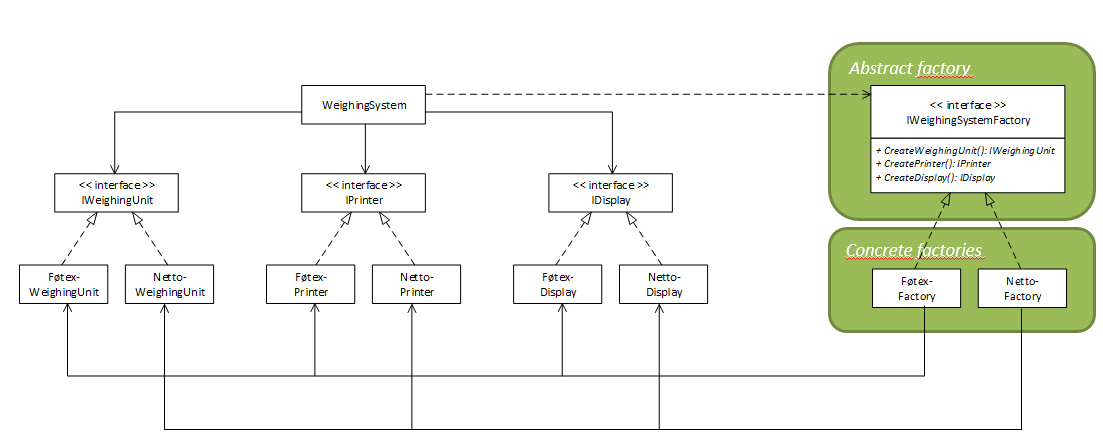
\includegraphics[width = \textwidth]{pics/usage_abstract_factory.PNG}
    \caption{Anvenselse af Abstract Factory}
    \label{fig:usage_abstract_factory}
\end{figure}

\begin{figure}[H]
    \centering
    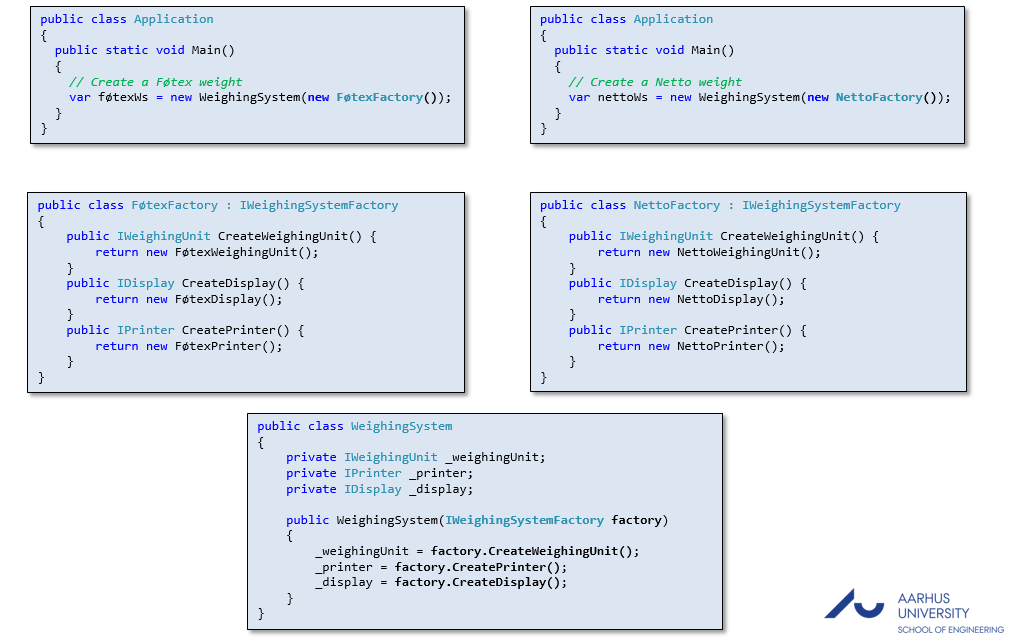
\includegraphics[width = \textwidth]{pics/abstract_factory_code.PNG}
    \caption{Abstract Factory Kode}
    \label{fig:abstract_factory_code}
\end{figure}



\end{document}
